%!TeX root=../tese.tex
%("dica" para o editor de texto: este arquivo é parte de um documento maior)
% para saber mais: https://tex.stackexchange.com/q/78101

\chapter{Projeto de Protocolo}

Agora que já definimos conceitos importantes e analisamos as principais implementações de protocolos de mensagens descentralizados, podemos definir um projeto de protocolo que possua parte das características anteriormente definidas. Este capítulo terá como objetivo explicar as decisões tomadas durante o projeto e quais limitações foram consideradas aceitáveis para o desenvolvimento de uma prova de conceito.

\section{Objetivos para o projeto}

Como não é possível cumprir todos os requisitos possíveis ao desenvolver um protocolo descentralizado, vamos precisar encontrar uma boa combinação de funcionalidades. Para este projeto, vamos considerar os seguintes requisitos:

\begin{itemize}
    \item \textbf{Simplicidade na configuração}: O protocolo não deve precisar de configurações avançadas de rede e deve funcionar em qualquer conexão residencial comum.
    \item \textbf{Pouca dependência em voluntários}: O protocolo deve ser razoavelmente resistente a maus atores e deve evitar depender de voluntários para funcionar.
    \item \textbf{Endereço de usuários estável}: O protocolo deve permitir que usuários tenham um endereço único e estável, para que possam ser identificados de maneira fácil.
    \item \textbf{Privacidade}: O protocolo deve evitar expor informações pessoais dos usuários e deve criptografar os dados do usuário quando possível.
\end{itemize}

Considerando esses requisitos, podemos já definir algumas características da nossa prova de conceito. 

\section{Proposta de arquitetura de rede}

Como discutido no primeiro capítulo, as arquiteturas dos protocolos de rede analisados podem ser divididas em quatro grupos diferentes: federados, indiretos por meio de \textit{relays} específicos da rede, indiretos por meio da rede do \textit{Tor} e \textit{peer-to-peer}. Podemos eliminar algumas dessas possibilidades com base nos requisitos que definimos.

Como consideramos que facilidade na configuração é um requisito importante, podemos concluir que não devemos desenvolver um serviço de arquitetura federada. Esse tipo de arquitetura depende de servidores mais centralizados ou que os usuários tenham conhecimento técnico e uma configuração de rede muito específica para que possam hospedar seu próprio servidor. Como buscamos um protocolo que consiga ser configurado sem esforço e que funcione em qualquer configuração de rede, vamos considerar outra arquitetura para esse projeto.

Queremos evitar que o protocolo seja muito dependente de \textit{relays} específicos da rede para funcionar. Esses \textit{relays} dependem de um serviço centralizado para que o usuário os encontre, e eles podem ser facilmente controlados por maus atores, especialmente quando o protocolo não possui muitos usuários. Como queremos que o protocolo não possua essas vulnerabilidades, não vamos desenhar o protocolo com essa arquitetura.

O protocolo do \textit{Tor} é uma opção interessante, pois ele é descentralizado e não depende de servidores específicos para funcionar. Ele possui grande quantidade de \textit{relays} voluntários, que vão continuar existindo independentemente do número de usuários utilizando este protocolo, e é bastante resistente a maus atores. Sua desvantagem é a quantidade de passos necessários para estabelecer uma conexão, o que gera uma latência maior. O \textit{Tor} também soluciona um problema muito grande da arquitetura \textit{peer-to-peer}, que é a dificuldade de encontrar outros usuários na rede, uma vez que endereços de IP residenciais são muitas vezes dinâmicos. Assim, vamos propor para esse projeto um programa de arquitetura híbrida, que utiliza o \textit{Tor} para encontrar outros usuários e uma arquitetura \textit{peer-to-peer} para a comunicação entre eles.

\subsection{Arquitetura de rede proposta: híbrida}

Na arquitetura proposta por este projeto, quando um usuário estiver \textit{online}, ele deve hospedar um serviço oculto com seu par de chaves público-privadas. O serviço oculto de cada usuário irá expor uma \textit{API} para outros usuários. Quando ele quiser realizar qualquer ação com outro usuário, ele deve conectar-se ao serviço oculto do outro usuário e utilizar algum dos \textit{endpoints} disponíveis. Esses \textit{endpoints} permitem diversas funcionalidades, como enviar mensagens, checar se o outro usuário o considera um "amigo" ou até mesmo solicitar uma conexão \textit{P2P} direta.

Consideramos que a privacidade é uma característica importante para o protocolo. Sabemos que a forma de comunicação por serviços ocultos proposta acima tem a grande vantagem de esconder o endereço IP de ambos os usuários, ao custo de maior latência. Enquanto algumas pessoas podem preferir se comunicar de forma anônima, outros usuários podem preferir conversar através de uma conexão direta, que é mais rápida e mais eficiente. Para isso, podemos propor um sistema de "amigos" para o protocolo. Quando um usuário considerar que prefere abrir mão de seu anonimato na conversa com outro usuário, ele pode escolher adicionar aquele endereço como amigo. Quando dois usuários são amigos, eles podem se comunicar diretamente, sem passar pelo serviço oculto. Isso permite que usuários que se conhecem e confiam um no outro possam se comunicar de forma mais eficiente, enquanto ainda mantêm a privacidade de usuários que não se conhecem.

Para evitar que o servidor do programa esteja constantemente monitorando outros usuários e tentando estabelecer uma conexão \textit{P2P}, podemos propor que toda vez que um usuário abre a conversa com outro, ele solicite uma conexão \textit{P2P}. Se ambos os usuários estiverem \textit{online}, ambos considerarem o outro como amigo, ambos estiverem com o \textit{chat} aberto com a outra pessoa e as configurações de rede permitirem, a conexão \textit{P2P} é estabelecida. Caso contrário, a comunicação é feita através do serviço oculto.

Esta solução permite que mensagens sejam enviadas em qualquer configuração de rede, permite que usuários se comuniquem de forma anônima, permite que os usuários se comuniquem de forma direta, não depende de \textit{relays} específicos da rede e é resistente a maus atores.

\section{Detalhes da implementação do protocolo}

A implementação desse protótipo foi organizada em torno de um único executável que lida com todos os aspectos do servidor. Este executável roda o \textit{Tor} como um subprocesso e sobe todos os \textit{endpoints} necessários para a comunicação entre usuários. Alguns desses \textit{endpoints} são acessíveis apenas localmente, enquanto outros serão acessíveis pela rede \textit{Tor}. A interface do usuário é feita através de um cliente \textit{web}, que se comunica com o executável através de uma \textit{API}.

Dada a experiência do autor dessa monografia com a linguagem de programação \textit{Python}, escolheu-se utilizá-la para o desenvolvimento do protótipo. \textit{Python} é uma linguagem de programação de alto nível, que possui uma grande quantidade de bibliotecas disponíveis para diversas funcionalidades. Além disso, \textit{Python} é uma linguagem de programação muito utilizada para desenvolvimento de aplicações \textit{web}, o que facilita a interação com a interface do usuário. O cliente \textit{web} é escrito em \textit{HTML}, \textit{CSS} e \textit{JavaScript}, e não utiliza nenhum \textit{framework} de \textit{frontend}.

Enquanto o servidor utiliza muitas bibliotecas, a principal é \textit{Flask}. \textit{Flask} é um \textit{framework web} minimalista para \textit{Python}, que permite a criação de aplicações \textit{web} de forma rápida e fácil. \textit{Flask} é muito utilizado para a criação de \textit{APIs} e é muito fácil de se utilizar.

\subsection{Servidor de \textit{backend}}

O servidor de \textit{backend} é composto por 12 arquivos, cada um com funções de um propósito específico.

\begin{itemize}
    \item \textbf{main.py}: Arquivo principal que inicializa o servidor e gerencia subprocessos.
    \item \textbf{\_\_init\_\_.py}: Vazio, utilizado para indicar que a pasta é um pacote \textit{Python}.
    \item \textbf{endpoints.py}: Inicializa todos os \textit{endpoints}, inicializa variáveis, e inicia o servidor de \textit{Flask}.
    \item \textbf{friends.py}: Contém muitas funções relacionadas a amigos, como \textit{requests} sobre amizades, pedidos de endereço de IP, pedidos de conexão \textit{P2P}, e funções relacionadas. Esses pedidos serão melhor explicados mais a frente.
    \item \textbf{jsonOperator.py}: Contém funções para ler e escrever todos os dados que o servidor precisa armazenar. O estado do programa é escrito em um arquivo \textit{json}. As funções de escrita utilizam um \textit{lock} para evitar condições de corrida.
    \item \textbf{middleware.py}: Tanto o tráfego do \textit{Tor} como o tráfego do cliente chegam à mesma \textit{API}. Para diferenciar entre os dois, utilizamos um \textit{middleware} que adiciona um \textit{header} "Tor-Middleware-Header", indicando se o \textit{request} veio do \textit{Tor} ou do cliente.
    \item \textbf{p2p.py}: Contém funções relacionadas à conexão direta entre participantes, seja por meio do \textit{localhost}, rede local, pela internet utilizando \textit{UPnP}, ou por meio de \textit{relays} do \textit{Tor}. É o arquivo mais complexo do servidor.
    \item \textbf{privateEndpoints.py}: Contém \textit{endpoints} que não devem ser acessíveis pela rede \textit{Tor}, como por exemplo de acesso às mensagens armazenadas, para envio de mensagens, ou para adicionar amigos.
    \item \textbf{publicEndpoints.py}: Contém \textit{endpoints} que devem ser acessíveis pela rede \textit{Tor}, como por exemplo para solicitar endereços de IP, solicitar conexões \textit{P2P}, ou para enviar mensagens.
    \item \textbf{serverCrypto.py}: Contém funções relacionadas à criptografia, como por exemplo assinaturas eletrônicas, criptografia de mensagens, e geração de chaves.
    \item \textbf{setup.py}: Contém funções para inicializar o \textit{Tor}, configurando portas, arquivos de configuração, e inicializando o processo.
    \item \textbf{upnp.py}: Contém funções para abrir portas no roteador do usuário, utilizando o protocolo \textit{UPnP}. Contém uma implementação própria porque a biblioteca de \textit{UPnP} para \textit{Python} não funcionou corretamente.
\end{itemize}
O servidor abre uma série de \textit{endpoints} locais e públicos, que são acessíveis pela rede \textit{Tor}. Os \textit{endpoints} públicos são:

\begin{itemize}
\item \textbf{pubEndpoint\_receiveMessage (POST)}: \textit{Endpoint} utilizado para receber mensagens de outros usuários. As mensagens são criptografadas de ponta a ponta pelo próprio protocolo do \textit{Tor} e são armazenadas no servidor.
\item \textbf{pubEndpoint\_getPublicKeyBase64 (GET)}: \textit{Endpoint} que retorna a chave pública do usuário em formato \textit{Base64}. Essa chave é utilizada para criptografar mensagens enviadas para o usuário e para verificar assinaturas digitais.
\item \textbf{pubEndpoint\_checkFriendRequest (POST)}: \textit{Endpoint} que verifica se há um pedido de amizade pendente de um determinado usuário.
\item \textbf{pubEndpoint\_getIpRequest (POST)}: \textit{Endpoint} que solicita o endereço IP de um usuário específico. Utilizado para tentar estabelecer uma conexão \textit{P2P}.
\item \textbf{pubEndpoint\_getFriendIP (POST)}: \textit{Endpoint} que retorna o endereço IP de um amigo, caso ambos os usuários tenham se adicionado como amigos.
\item \textbf{pubEndpoint\_p2pRequest (GET)}: \textit{Endpoint} que solicita o estabelecimento de uma conexão \textit{P2P} direta entre dois usuários.
\item \textbf{pubEndpoint\_receiveGenericFriendRequest (POST)}: \textit{Endpoint} utilizado para receber pedidos genéricos de amizade de outros usuários.
\item \textbf{pubEndpoint\_ping (GET)}: \textit{Endpoint} utilizado para verificar se o servidor está \textit{online} e respondendo às requisições.
\end{itemize}

Os \textit{endpoints} locais são:

\begin{itemize}
\item \textbf{privEndpoint\_getMessagesFromSender (POST)}: \textit{Endpoint} utilizado para obter mensagens de um remetente específico.
\item \textbf{privEndpoint\_sendMessage (POST)}: \textit{Endpoint} utilizado para enviar mensagens para outros usuários.
\item \textbf{privEndpoint\_getLatestMessages (GET)}: \textit{Endpoint} utilizado para obter as mensagens mais recentes.
\item \textbf{privEndpoint\_getSenders (GET)}: \textit{Endpoint} utilizado para obter a lista de remetentes.
\item \textbf{privEndpoint\_getAddress (GET)}: \textit{Endpoint} utilizado para obter o endereço do usuário.
\item \textbf{privEndpoint\_startChat (POST)}: \textit{Endpoint} utilizado para iniciar uma conversa com outro usuário.
\item \textbf{privEndpoint\_getFriends (GET)}: \textit{Endpoint} utilizado para obter a lista de amigos.
\item \textbf{privEndpoint\_addFriend (POST)}: \textit{Endpoint} utilizado para adicionar um amigo.
\item \textbf{privEndpoint\_removeFriend (POST)}: \textit{Endpoint} utilizado para remover um amigo.
\item \textbf{privEndpoint\_changeFocusedFriend (POST)}: \textit{Endpoint} utilizado para mudar o amigo focado na interface.
\item \textbf{privEndpoint\_getFriendConnectionStatus (GET)}: \textit{Endpoint} utilizado para obter o status de conexão de um amigo.
\end{itemize}

\subsection{Cliente \textit{web}}

O cliente \textit{web} é composto por uma aba de conversas e uma aba de amigos. A aba de conversas mostra uma lista com todas as pessoas com as quais o usuário já conversou e permite que o usuário selecione uma conversa para visualizar. A aba de amigos mostra uma lista com todos os amigos do usuário e permite que o usuário adicione ou remova amigos.

Como o cliente não é o escopo principal deste projeto, ele é simples e apenas cumpre os requisitos necessários ao projeto. As imagens \ref{fig:mensagens}, \ref{fig:amigos} e \ref{fig:home} mostram respectivamente a conversa entre dois usuários, a aba que contém os amigos do usuário e a aba principal da interface.

\begin{figure}[H]
    \centering
    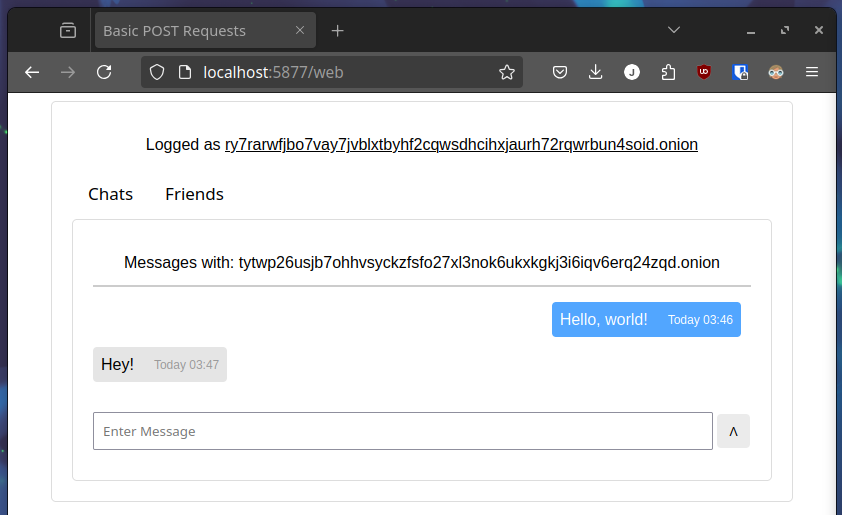
\includegraphics[width=0.7\textwidth]{mensagens.png}
    \caption{Captura de tela da interface mostrando a conversa entre dois usuários.}
    \label{fig:mensagens}
\end{figure}

\begin{figure}[H]
    \centering
    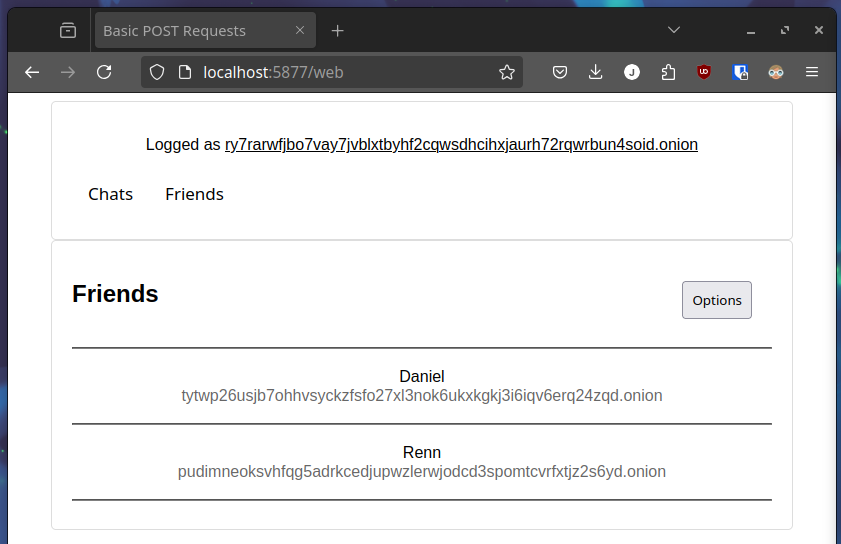
\includegraphics[width=0.7\textwidth]{amigos.png}
    \caption{Captura de tela da aba que contém os amigos de um dado usuário.}
    \label{fig:amigos}
\end{figure}

\begin{figure}[H]
    \centering
    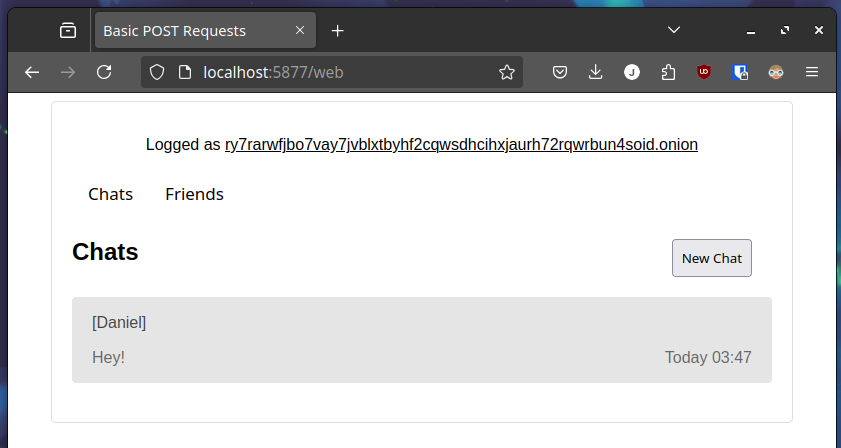
\includegraphics[width=0.7\textwidth]{home.png}
    \caption{Captura de tela da aba principal da interface, contendo todas as conversas de um dado usuário.}
    \label{fig:home}
\end{figure}

\section{Criptografia e \textit{handshakes}}

O servidor utiliza alguns métodos de criptografia para garantir a segurança das mensagens trocadas entre os usuários. A intenção inicial do projeto era que o servidor utilizasse a mesma chave pública e privada que o subprocesso do \textit{Tor}, porém, como o \textit{Tor} usa regras de derivação de chave diferentes das da biblioteca \textit{ED25519}\footnote{ED25519 é um esquema de assinatura digital e criptografia de chave pública baseado no algoritmo de curva elíptica Edwards. Ele permite que mensagens sejam assinadas e sua autenticidade seja verificada, e permite que usuários criptografem mensagens para outros usuários, apenas tendo acesso a chave pública do destinatário.} do \textit{Python}, os servidores vão compartilhar chaves privadas, mas vão utilizar chaves públicas diferentes para acessar o \textit{Tor} e para assinar e criptografar mensagens. Isto poderia gerar um problema de verificação de autenticidade da chave pública, uma vez que o protocolo do \textit{Tor} garante a autenticidade de uma chave pública realizando a derivação do endereço a partir da chave pública, permitindo que, ao acessar um serviço oculto, o usuário tenha certeza de que a chave pública que ele recebeu está correta. Assim, o primeiro contato entre dois servidores teve que ser repensado para garantir que ambos os usuários consigam assegurar que têm a chave pública correta de seus amigos.

Sabemos que, ao acessar um serviço oculto, o \textit{Tor} realiza a verificação da chave pública recebida. Assim, sabemos que, quando queremos iniciar uma conversa com um usuário novo, podemos simplesmente acessar o \textit{endpoint} \textit{pubEndpoint\_getPublicKeyBase64} do usuário, e o \textit{Tor} irá garantir que a chave pública que recebemos é a correta. Porém, como garantir que a chave pública que recebemos é a correta quando recebemos uma mensagem de um usuário com o qual nunca falamos antes? Para resolver esse problema, propomos um \textit{handshake} inicial entre os dois servidores.

Quando o servidor receber um pedido de envio de mensagem de um usuário com o qual ele nunca falou antes, ele irá responder a esse pedido de envio de mensagem com a mensagem "refaça esse envio, vou pedir sua chave pública primeiro". O servidor então irá acessar o \textit{endpoint} \textit{pubEndpoint\_getPublicKeyBase64} da pessoa que está enviando a mensagem, e assim que receber esse \textit{request} novamente, irá verificar se a chave pública recebida é a mesma que a chave pública que ele recebeu anteriormente. Esse processo acontece de forma síncrona, de modo que o segundo pedido de envio de mensagem demorará um pouco para ser respondido, sendo completado quando o servidor tiver certeza de que a chave pública recebida é a correta.

Uma vez que ambos os servidores têm chaves públicas com autenticidade confirmada, eles podem assinar mensagens, criptografar mensagens e verificar assinaturas digitais.

A criptografia de mensagens não é necessária quando os usuários estão conversando através do \textit{Tor}, uma vez que o protocolo do \textit{Tor} já criptografa as mensagens de ponta a ponta. Porém, quando os usuários estão conversando de forma direta, a criptografia é necessária.

\subsection{Pedidos exclusivos para amigos}

Alguns pedidos entre servidores requerem uma "prova" de autenticidade. Por exemplo, caso o usuário A queira pedir o endereço IP do usuário B, ele deve provar que é amigo de B. Pedidos como esse têm um formato padronizado e são gerados e verificados no arquivo \textit{friends.py}. O servidor que recebe o pedido verifica se o pedido é válido e, se for, responde com a informação solicitada. O formato de cada pedido é o seguinte:

\begin{itemize}
    \item \textbf{origin}: Endereço do usuário que está fazendo o pedido.
    \item \textbf{destination}: Endereço do usuário que está recebendo o pedido.
    \item \textbf{timestamp}: Hora exata em que o pedido foi feito.
    \item \textbf{kind}: Tipo de pedido que está sendo feito.
    \item \textbf{signature}: Assinatura digital do pedido, gerada a partir do \textit{JSON} do pedido.
\end{itemize}

Dessa maneira, pedidos não podem ser reutilizados e pedidos não podem ser feitos em nome de outro usuário.

\section{\textit{Handshake} \textit{P2P}}

Quando um usuário abre uma conversa na interface, o servidor vai seguir uma série de passos para determinar se uma conexão direta entre usuários pode ser feita.
\begin{enumerate}
    \item O servidor verifica se os usuários são amigos mútuos.
    \item O servidor espera que o outro usuário também tenha esta conversa aberta.
    \item O servidor pede os endereços IP do outro usuário.
    \item Se os usuários tiverem endereços IP públicos e privados iguais, ele tenta estabelecer uma conexão pelo \textit{localhost}.
    \item Se os usuários tiverem endereços IP públicos iguais e endereços IP privados diferentes, ele tenta estabelecer uma conexão pela rede local.
    \item Se os usuários tiverem endereços IP públicos diferentes, ele tenta estabelecer uma conexão direta entre eles usando \textit{UPnP}.
\end{enumerate}

Caso qualquer um desses passos não seja bem-sucedido, os usuários ainda poderão comunicar-se normalmente usando o \textit{Tor} como intermediário.

\section{Considerações finais}

A implementação do protocolo não é um produto finalizado e não deve ser utilizada como um substituto para programas de envio de mensagens popularmente utilizados. Embora ele consiga cumprir os requisitos que foram propostos, ele não foi testado extensivamente no mundo real e provavelmente é vulnerável a ataques. Ainda assim, ele é uma demonstração muito interessante de um tipo de arquitetura que não foi muito explorado por projetos acadêmicos até agora. O protocolo foi implementado como software livre seguindo a licença \textit{GNU GPL v3} e está disponível publicamente em \url{https://linux.ime.usp.br/~renner/MAC0499/} (hospedado pela infraestrutura da USP) e \url{https://github.com/LeRenner/mac0499-prototype} (hospedado por um serviço externo). O código deste programa contém dependências disponíveis por meio de outras licenças. O arquivo /LICENÇA.txt contém uma lista de todas as dependências e suas licenças.